\documentclass[10pt,a4paper]{article}


%%%%%%%%%%%%%%%%%%%%PACKAGES%%%%%%%%%%%%%%%%%%%%
\usepackage{color}  % add colors to text
\usepackage{microtype} %better letter spacing and etc
\usepackage{titling} %control the typeset of maketitle
\usepackage{lipsum} %get that sweet lorem ipsum text
%\usepackage[11pt]{moresize}

\usepackage{float} %allows strict placement of a float + override latex replacement -->use H

\usepackage{graphicx} %import graphs images and whatnot
\usepackage{tikz} %graphic elements + drawing power over 9000; be careful with semi-column syntax
\usetikzlibrary{calc} %for operations on tikz elements
% http://www.texample.net/tikz/examples/feature/absolute-positioning/
\usepackage{amsmath}  %pimp your equations
\usepackage{amssymb}  %all those extra math symbols
\usepackage{siunitx} 	% SI units

%\usepackage[francais]{babel} %language it's gonna be loaded in
\usepackage[english]{babel}
%\usepackage[utf8]{inputenc} 
\usepackage[T1]{fontenc}  %font encoding of the input text

%\usepackage[colorlinks,bookmarks=false,citecolor=black,linkcolor=blue,urlcolor=blue]{hyperref}


\usepackage{pgfplots} 	% plot directly in latex
\pgfplotsset{compat=1.13} %backwards compatibility mode (pgfplots regularly updated)
 
\usepackage{caption}  %customize figure captions
\usepackage{subcaption}  %create multiple floats within a single environment giving individual captions

\usepackage{tabularx} % x designator for auto expanding width of a table column
\usepackage{tabulary} %better columns for tables: l c r j
\usepackage{booktabs} %get those pretty tables
\usepackage{booktabs} %extra commands for creating stylish tables
\usepackage{arydshln} %drawing dash lines in arrays/tabulars

\usepackage{array}  %more table handling
\usepackage{multirow} %typeset text into multiple rows
\usepackage{wrapfig} %figures with which text can flow around

\usepackage{verbatim} %good for bug fixes and commenting on code
\usepackage{verbdef} % http://ctan.org/pkg/verbdef



%%%%%%%%%%%%%%%%%%%%PAGE FORMATTING AND WHAT NOT%%%%%%%%%%%%%%%%%%%%
\usepackage[twocolumn,hmargin=2cm,vmargin=2.5cm]{geometry}% rm if title --> full width span when 2column format
%\usepackage[top=2.5cm, bottom=1.5cm, left=2cm, right=2cm]{geometry} %document margin and page size
%\addtolength{\oddsidemargin}{-1cm}
%\addtolength{\evensidemargin}{-1cm}
%\addtolength{\textwidth}{1cm}
%\addtolength{\topmargin}{-1cm}
%\addtolength{\textheight}{1cm}
%\paperheight=297mm
%\paperwidth=210mm
%\setlength{\textheight}{235mm}
%\setlength{\topmargin}{-1.2cm}
%\setlength{\footskip}{5mm}
%\setlength{\textwidth}{15cm}
%\setlength{\oddsidemargin}{-0.56cm}
%\setlength{\evensidemargin}{-0.56cm}


%%%%%%%%%%%%%%%%%%%%MACRO DOODLES%%%%%%%%%%%%%%%%%%%%

%\makeatletter %make @ usable for macro name: catcode 12--> 11 to access internal macros
%\renewcommand{\section}{\@startsection {section}{1}{\z@}%
%             {-3.5ex \@plus -1ex \@minus -.2ex}%
%             {2.3ex \@plus.2ex}%
%             {\normalfont\normalsize\bfseries}}
%\makeatother %switch @ back to catcode 11-->12 


%%%%%%%%%%%%%%%%%%%%ABREVIATIONS AND DEFINITIONS%%%%%%%%%%%%%%%%%%%%

\def \tss {\textsuperscript}



%%%%%%%%%%%%%%%%%%%%PATHS%%%%%%%%%%%%%%%%%%%%

\graphicspath{{../src/}}



%%%%%%%%%%%%%%%%%%%%DOCUMENT%%%%%%%%%%%%%%%%%%%%
%	
\includegraphics[scale=0.1]{epfllogo.png}\\

\title{
	\vspace*{-1.3cm}
	
\includegraphics[scale=0.1]{epfllogo.png}\\
	\vspace*{0.3cm}
	\large{\textbf{Higgs Boson Machine Learning Challenge}}}
	
\date{\normalsize{\today}} %date of report: 29/10/2018
%\author{Bian Theophile, Guillain Leonore, Mercan Samuele}
\author{\normalsize{Th\' eophile 	\sc{Bian}} \and \normalsize{L\' eonore \sc{Guillain}} \and \normalsize{Samuele \sc{Mercan}}}

\begin{document}
\maketitle
%\begin{tikzpicture}[remember picture, overlay]
%\node [shift={(-3.8cm, -1cm)}] at (current page.north east) {
\includegraphics[scale=0.08]{epfllogo.png}};
%ax\node[anchor= south east] at (current page.south east) {
\includegraphics[scale=0.06]{epfllogo.png}};
%\end{tikzpicture}

%\vspace*{-1cm}

\paragraph{Abstract:} This report was written in the scope of an EPFL Machine Learning Course, for a project based on the Higgs Boson Kaggle competition (2014). The main objective of this work is to create a binary classifier that is able to differentiate in between the decay of a Higgs boson into fermion pairs and background signals -- recordings of other particles in the quantic standard model as well as measurement noise. The data set used was simulated by the ATLAS experiment, and was used to optimize measurement. Recorded events are characterized by 30 features, which are used to classify it as a signal of interest or as background. As some of the features depend on the type of decay occuring, they are not always defined\footnote{C. Adam-Bourdarios et al.(2015), \textit{The Higgs Boson Machine Learning Challenge}, Proceedings of Machine Learning Research}. Therefore some values are set to be out-of-range in a physical sense or not derivable -- the actual value is set to -999.0 for easier manipulation. After data exploration and preprocessing we evaluated different regression and classification methods using cross-validation. After having chosen a model based on predictive accuracy and implementation considerations, we adjusted it to include feature expansion in order to improve our predictions.
	
\paragraph{Data Exploration:}Data exploration is a crucial step towards building an efficient model. First we split the given 250'000 events dataset into two sets with a 9:1 ratio. The largest set was subsequently divided using the same ratio to be able to evaluate our models through 10-fold cross-validation, creating a training and a test set. The remaining 10\% of the initial dataset is grouped into a mock submission set to avoid overfitting with the Kaggle test set. We checked the mean, the standard deviation and the distribution of each feature in the training set. As a first approach we decided to handle out-of-range values by assigning them a "Not a Number" tag (NaN), and computed the percentage of NaNs for each feature (cf. Fig.1). We also removed these values to see how each feature distribution changes. As these values have a strong impact on data distribution, observations made without handling them are often unreliable. We graphically assessed that some feature distributions are strongly left-skewed. In order to confirm our intuition we used QQ-plotting on each distribution; the left-skewness of data was consistent. We also applied a correlation test on features to evaluate whether they were independent or not.

\paragraph{Baseline Model:}The baseline model used a least squares regression method, as it is not prone to overfitting and is adapted to the data set; computing the rank of our data matrix showed that it is well-conditioned. Data points, including out of range values were standardized feature-wise and used in the algorithm. In our initial model, we observed from the weight distribution that NaN-containing features were not essential to the prediction. To verify our approach, we evaluated different methods against each other and found that changing the out-of-range values to equal the mean or changing them to equal zero doesn't noticeably affect the prediction accuracy. Removing all out of range-containing features yielded poorer accuracy, therefore we decided to replace these values with the mean of the feature (evaluated without the out-of-range values). 

\paragraph{Model 1:}Moving forward, we added one-hot encoding to the jet number values -- corresponding to the only categorical feature -- using L2 regularization. \\
\indent The algorithm was executed iteratively over a range of values for the learning rate hyperparameter to find the optimal setting, and starting weights were set to zero to maximize algorithm efficiency. We tested $\gamma$ values from $e^{-4}$ to $e^{1}$. Then we tried values of 100, 200 and 500 for the maximum number of iterations and did not see marked difference between them so we opted for the smaller one for computational complexity reasons. The ultimate stage of the model was to use logistic and regularized logistic regression. The accuracy of our different baseline models gave us insight as to which one should be preferred for later additions.

\paragraph{Model 2:}The next model's key addition was splitting data points by jets, which yields four different subsets pertaining to jet numbers 0, 1, 2 and 3 (Model 2.a). Feature engineering was the following extension to the model; namely polynomial base expansion of our features, this time using a Ridge-regression instead of least-squares regression to counter overfitting (Models 2.b and 2.c). We decided to use Ridge-regression because stochastic gradient descent is too computationally costly considering the range over which we have to test our hyperparameters. We tested different polynomial bases from degree 1 to 14 separately for each jet subset (cf. Fig.2).\\
\indent We also added new features corresponding to the logarithmic transformation of each feature that showed a left-skewed distribution. A first implementation of this idea led us to replace the initial features, while in a second implementation we added new logarithmic features while keeping the original features (Model 2.d). Results are summarized in Tab.1.\\
\indent We also took mean square error into consideration to be able to better our models. However as the model gets more complex, it tends to produce larger errors even when the prediction is correct. While the error increased, the accuracy also increased and our model showed no signs of overfitting, no marked drop of accuracy in independent dataset testing, and the variance of the accuracy was reasonably low.

\paragraph{Optimal Submission:}Data was normalized and separated (4 subsets; jet number $= 0, 1, 2, 3$) as previously detailed. We used feature augmentation; adding $x*y$ features when below a 0.05 correlation threshold as well as polynomial basis expansion with polynomial degrees of 12, 12, 14 and 12 for jet number subsets 0, 1, 2 and 3 respectively. Using Ridge-regression with a learning-rate of $\lambda = 0.001$ we obtained an accuracy of 0.83251\% on the Kaggle submission (Model 2.c).

\paragraph{Discussion:}It is vital to verify that adding features while using a least squares regression method does not lead to ill-conditioning of the data matrix. However, since feature expansion is needed for an accurate prediction, it might be best to use another model, such as Ridge-regression. Furthermore the fact that $x*y$ feature expansion improves our results (increase of 1\% after cross-featuring) justifies the feature expansion approach; in fact cross-features are at the core of the competition's best algorithms\footnote{Bernard Ong et al. (2016), textit{What It Took to Score the Top 2\% on the Higgs Boson Machine Learning Challenge}, NYC Data Science Academy}. Using neural network models allows to test for different relationships between features, whereas we only tested for multiplicative two-variable relationship. On the other hand, we also observed that not all feature expansion methods are always appropriate; both our logarithm feature transformation did not improve our score as they increased our algorithm's tendency to overfit.\\
\indent Our choice to use a Ridge-regression is in part explained by the fact that other methods are more computationally demanding (e.g. regularized logistic regression). Having tested different regression methods early on, we observed that Ridge-regression fared as well as regularized logistic regression. However these results might be different after more intensive data preprocessing. Moving forward, we should consider investigating different models as well as continuing to improve our Ridge-regression model. While it is a limited model as previously discussed, it is simple and efficient enough to be of interest for future additions. Using additional data processing methods such as Principal Component Analysis could allow removal of features that are not essential in the predictive algorithm, therefore allowing us to test additonal feature transformations while keeping the computation cost low.\\
\vspace*{0cm}
\normalsize{\textbf{Figures:}}
\vspace*{0cm}
\begin{figure}[H]
\begin{center}
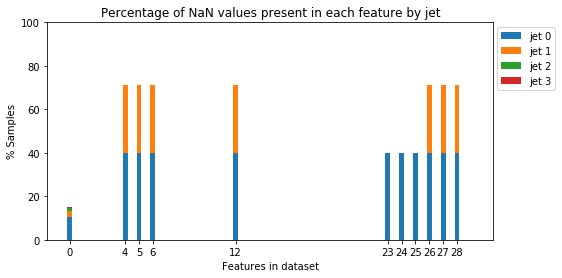
\includegraphics[scale=0.45, trim=0cm 0cm 0cm 0cm, clip=true]{nanCount2.png}
\caption{\label{Fig.1}Percentage of NaN values present in each feature by jet}
\end{center}
\textit{\footnotesize{Out-of-range values are labeled as NaNs in order to better understand their importance. \textbf{Fig.1} shows that these values are mainly contained within the jet subsets 0 and 1, as these features are not defined for jet numbers below 2. After further exploration, we know that only the first feature (left-most) has out-of-range values for all jet subsets; this is caused by measurement limitations.}}
\end{figure}
\vspace*{0.20cm}

 	 	
\begin{table}[hbtp]
\begin{center}
\begin{tabular}{l|c|c|c}
%\toprule
\textbf{Model 2.a} & \textbf{Model 2.b} & \textbf{Model 2.c} & \textbf{Model 2.d} \\
\midrule
0.75889\% & 0.82464\% & 0.83251\% & 0.73258\% \\
%\bottomrule
\end{tabular}
\caption{\label{Tab.1}Model comparison based on prediction accuracy}
\end{center}
\footnotesize{\textbf{Tab.1} \textit{shows prediction accuracy for different models:}
Model 2.a: \textit{Least Squares Regression, jet separation;}
Model 2.b: \textit{Ridge Regression, jet separation, polynomial basis feature expansion;}
Model 2.c: \textit{Improvements on Model 2.b: Fine-tuning of hyperparameters, cross-featuring;}
Model 2.d: \textit{Modifications on Model 2.b: logarithmic transformation of some features}}
\end{table}
\vspace*{0.20cm}


\begin{figure}[H]
\begin{center}
%\includegraphics[trim=0cm 0.65cm 0cm 0.65cm, clip=true,width=\linewidth]{}
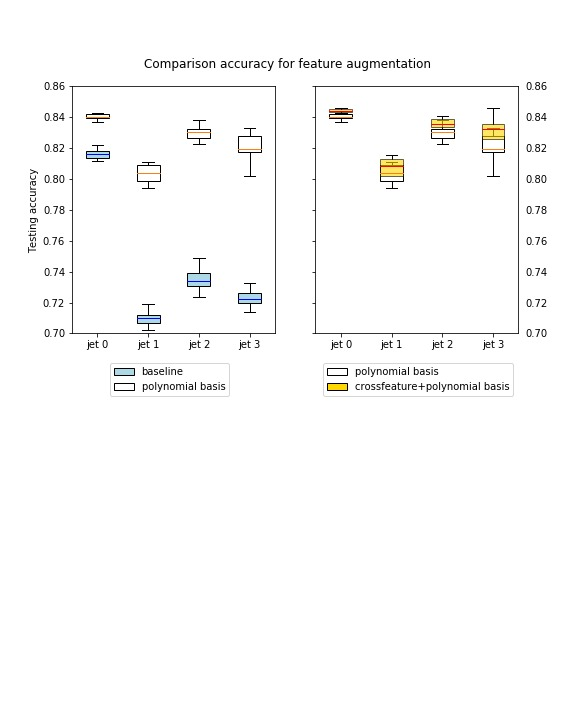
\includegraphics[scale=0.45,trim=0cm 11cm 0cm 2cm, clip=true]{featureAccuracy3.jpeg}
\caption{\label{Fig.2}Comparison of accuracy on data subsets in between feature augmentation models}
\end{center}
\textit{\footnotesize{\textbf{Fig.2} shows an improvement of our prediction accuracy throughout all subsets when using polynomial basis expansion. Furthermore, cross-feature expansion also shows improved accuracy when combined with the polynomial basis expansion.}}
\end{figure}

\end{document}	\grid
\grid
\grid
\grid
